    % --- IMPORTS ---
	\documentclass[leqno]{article}
	\usepackage{graphicx}
	\usepackage{dsfont}
	\usepackage{mathtools}
	\usepackage{amssymb}
	\usepackage{amsmath}
	\usepackage{amsthm}
	\usepackage{float}
	\usepackage{ragged2e}
	\usepackage{tensor}
	\usepackage{fancyhdr}
	\usepackage{empheq}
	\usepackage[most]{tcolorbox}
	\usepackage{enumitem}
	\usepackage{dirtytalk}
	\usepackage{marginnote}
	\usepackage{microtype}
	\usepackage[
	  a4paper,
	  left=0.8in,
	  right=1in,
	  top=1in,
	  bottom=0.5in,
	  headheight=14pt,
	  headsep=0.4in
	]{geometry}
	\setlength{\parindent}{0cm}
	% --- TikZ Packages ---
	\usepackage{pgfplots}
	\pgfplotsset{compat=1.18}
	\usepgfplotslibrary{fillbetween, polar}
	\usetikzlibrary{calc, positioning}
	\usetikzlibrary{angles, quotes}
	\usetikzlibrary{arrows.meta}
	\usetikzlibrary{decorations.pathreplacing, decorations.markings}
	\usetikzlibrary{patterns}
	\usetikzlibrary{intersections}
	% --- URL Packages ---
	\usepackage[colorlinks=true,linkcolor=red,citecolor=magenta,urlcolor=black]{hyperref}%
	\urlstyle{same}
	% --- END OF IMPORTS ---
	
	% --- CUSTOM COMMANDS ---
	\RenewDocumentCommand{\marks}{o m}{%
	  \IfValueTF{#1}%
		{\marginnote{\raggedright\textbf{[#2]}}[#1]}%
		{\marginnote{\raggedright\textbf{[#2]}}}%
	}
	\newcommand{\vspacerule}[2]{%
	  \par\vspace*{#1}%
	  \noindent\hrulefill\par
	  \vspace*{#2}%
	}
	\definecolor{scarlet}{RGB}{205, 40, 75}
	\newcommand{\questionitem}{%
	  \item\phantomsection
	  \addcontentsline{toc}{section}{Question \number\value{enumi}}%
	}
	\renewcommand{\contentsname}{Questions}
	% --- END OF CUSTOM COMMANDS ---
	
	% --- HEADER CONFIG ---
	\pagestyle{fancy}
	\fancyhead{}
	\fancyfoot{}
	\renewcommand{\headrulewidth}{0.9pt}
	\lhead{\textit{Solutions} - Integration of Polar Curves}
	\chead{}
	\rhead{\href{https://danieljsmith.org}{danieljsmith.org}}
	% --- END OF HEADER CONFIG ---
	
	\begin{document}
	\vspace*{20pt}
	\tableofcontents
	\newpage
	\begin{enumerate}[
	  label=\textbf{\arabic*.},
	  leftmargin=*,
	  topsep=0pt,
	  partopsep=0pt,
	  parsep=0pt
	]
	
% ---- Question 1 ----
\questionitem
% [Source: _QBT__Integration_of_Polar_Curves, Q1]

\begin{figure}[H]
    \centering
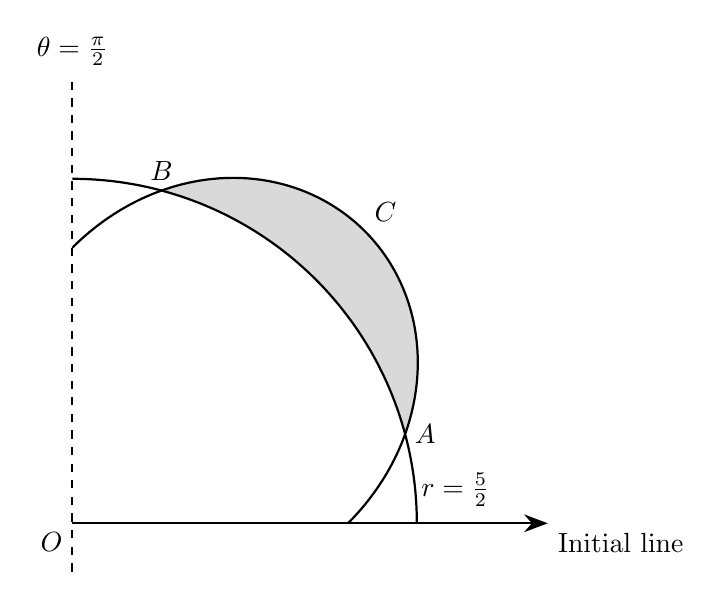
\begin{tikzpicture}[scale=1.75]
\def\R{2.5}
\def\thA{15}
\def\thB{75}

\coordinate (O) at (0,0);
\coordinate (A) at (\thA:\R);
\coordinate (B) at (\thB:\R);
\coordinate (Clab) at ({(2+sin(2*45))*cos(45)},{(2+sin(2*45))*sin(45)});
\coordinate (Dlab) at ({1*\R*cos(10)},{1.*\R*sin(10)});

\draw[dashed, thick] (0,-0.35) -- (0,3.25);
\node[above] at (0,3.25) {$\theta=\frac{\pi}{2}$};

\draw[-{Stealth[length=3mm]}, thick] (0,0) -- (3.45,0) node[below right] {Initial line};

\fill[gray!30]
  plot[smooth, samples=140, domain=\thA:\thB]
    ({(2+sin(2*\x))*cos(\x)},{(2+sin(2*\x))*sin(\x)})
  --
  plot[smooth, samples=140, domain=\thB:\thA]
    ({\R*cos(\x)},{\R*sin(\x)})
  -- cycle;

\draw[thick]
  plot[smooth, samples=160, domain=0:90]
    ({\R*cos(\x)},{\R*sin(\x)});

\draw[thick]
  plot[smooth, samples=220, domain=0:90]
    ({(2+sin(2*\x))*cos(\x)},{(2+sin(2*\x))*sin(\x)});

\node[below left] at (O) {$O$};
\node[right] at (A) {$A$};
\node[above] at (B) {$B$};
\node[above right] at (Clab) {$C$};
\node[below right] at (Dlab) {$r=\frac{5}{2}$};
\end{tikzpicture}
\end{figure}


The diagram shows part of the curve $C$ with polar equation
\[
r=2+\sin 2\theta,\quad 0\leq\theta\leq\frac{\pi}{2}
\] \\
and the circle
\[
r=\frac{5}{2}
\] \\
The curve and the circle intersect at the points $A$ and $B$, as shown. \\

Find, correct to three significant figures, the area of the shaded region enclosed by $C$ and the circle. \marks{9} \\

	\vspace*{10pt}
	
	\begin{tcolorbox}[colback=white, colframe=scarlet, title={\textbf{Solution}}, breakable, grow to left by=6mm, grow to right by=10mm]
	For the intersection points of the curve and the circle, set the two values of $r$ equal:
	
	\[
	2+\sin 2\theta=\frac52
	\]
	
	So
	
	\[
	\sin 2\theta=\frac12
	\]
	
	Since $0\le \theta \le \frac{\pi}{2}$, we have $0\le 2\theta \le \pi$, so the solutions are
	
	\[
	2\theta=\frac{\pi}{6},\ \frac{5\pi}{6}
	\]
	
	Hence
	
	\[
	\theta=\frac{\pi}{12},\ \frac{5\pi}{12}
	\]
	
	So the points of intersection are at $\theta=\frac{\pi}{12}$ and $\theta=\frac{5\pi}{12}$.
	
	For $\frac{\pi}{12}\le \theta \le \frac{5\pi}{12}$, we have $\sin 2\theta \ge \frac12$, so
	
	\[
	2+\sin 2\theta \ge \frac52
	\]
	
	Therefore the curve $C$ lies outside the circle on this interval, and the required area is
	
	\[
	A=\frac12\int_{\pi/12}^{5\pi/12}\left[\left(2+\sin 2\theta\right)^2-\left(\frac52\right)^2\right]\mathrm{d}\theta
	\]
	
	Now expand the integrand:
	
	\begin{align*}
	A&=\frac12\int_{\pi/12}^{5\pi/12}\left(4+4\sin 2\theta+\sin^2 2\theta-\frac{25}{4}\right)\mathrm{d}\theta\\
	&=\frac12\int_{\pi/12}^{5\pi/12}\left(-\frac94+4\sin 2\theta+\sin^2 2\theta\right)\mathrm{d}\theta
	\end{align*}
	
	Use the identity
	
	\[
	\sin^2 2\theta=\frac{1-\cos 4\theta}{2}
	\]
	
	Then
	
	\begin{align*}
	A&=\frac12\int_{\pi/12}^{5\pi/12}\left(-\frac94+4\sin 2\theta+\frac{1-\cos 4\theta}{2}\right)\mathrm{d}\theta\\
	&=\frac12\int_{\pi/12}^{5\pi/12}\left(-\frac74+4\sin 2\theta-\frac12\cos 4\theta\right)\mathrm{d}\theta
	\end{align*}
	
	Integrating,
	
	\begin{align*}
	A&=\left[-\frac{7\theta}{8}-\cos 2\theta-\frac{1}{16}\sin 4\theta\right]_{\pi/12}^{5\pi/12}
	\end{align*}
	
	Now substitute the limits:
	
	\begin{align*}
	A&=\left(-\frac{35\pi}{96}-\cos\frac{5\pi}{6}-\frac{1}{16}\sin\frac{5\pi}{3}\right)
	-\left(-\frac{7\pi}{96}-\cos\frac{\pi}{6}-\frac{1}{16}\sin\frac{\pi}{3}\right)
	\end{align*}
	
	Using
	\[
	\cos\frac{5\pi}{6}=-\frac{\sqrt3}{2},\quad
	\sin\frac{5\pi}{3}=-\frac{\sqrt3}{2},\quad
	\cos\frac{\pi}{6}=\frac{\sqrt3}{2},\quad
	\sin\frac{\pi}{3}=\frac{\sqrt3}{2}
	\]
	
	gives
	
	\begin{align*}
	A&=\left(-\frac{35\pi}{96}+\frac{\sqrt3}{2}+\frac{\sqrt3}{32}\right)
	-\left(-\frac{7\pi}{96}-\frac{\sqrt3}{2}-\frac{\sqrt3}{32}\right)\\
	&=-\frac{28\pi}{96}+\frac{34\sqrt3}{32}\\
	&=-\frac{7\pi}{24}+\frac{17\sqrt3}{16}
	\end{align*}
	
	So the exact area is
	
	\[
	A=\frac{17\sqrt3}{16}-\frac{7\pi}{24}
	\]
	
	and numerically
	
	\[
	A\approx 0.924
	\]
	
	Therefore, the area of the shaded region is $0.924$ square units, correct to three significant figures.
	\end{tcolorbox}
	
	
	\newpage
	
% ---- Question 2 ----
\questionitem
% [Source: _QBT__Integration_of_Polar_Curves, Q2]

\begin{enumerate}[label=\textbf{(\alph*)}]
  \item A curve has polar equation $r=a\sin^23\theta$, where $a>0$ and $0\leq \theta<2\pi$. \\
  \begin{enumerate}[label=(\roman*)]
    \item Sketch the curve. \marks{2} \\
    \item Find, in exact form, the total area of the regions enclosed by the curve. \marks{7} \\
  \end{enumerate}
\end{enumerate}

	\vspace*{10pt}
	
	\begin{tcolorbox}[colback=white, colframe=scarlet, title={\textbf{Solution}}, breakable, grow to left by=6mm, grow to right by=10mm]
	\begin{enumerate}[label=\textbf{(\alph*)}]
	  \item
	  \begin{enumerate}[label=(\roman*)]
		\item Since
		\[
		r=a\sin^2(3\theta)
		\]
		we have $r\geq 0$ for all $\theta$.
	
		Also,
		\[
		\sin^2(3(\theta+\tfrac{\pi}{3}))=\sin^2(3\theta+\pi)=\sin^2(3\theta)
		\]
		so the curve has period $\tfrac{\pi}{3}$. Hence the part from $0\leq \theta<\tfrac{\pi}{3}$ repeats 6 times as $\theta$ goes from $0$ to $2\pi$.
	
		The curve passes through the pole when
		\[
		\sin^2(3\theta)=0 \quad \Rightarrow \quad 3\theta=n\pi \quad \Rightarrow \quad \theta=\frac{n\pi}{3}
		\]
		for $n=0,1,2,3,4,5$.
	
		The maximum value of $r$ is $a$, and this occurs when
		\[
		\sin^2(3\theta)=1 \quad \Rightarrow \quad 3\theta=\frac{\pi}{2}+n\pi
		\]
		so
		\[
		\theta=\frac{\pi}{6}+\frac{n\pi}{3}
		\]
		for $n=0,1,2,3,4,5$.
	
		So the curve is a 6-petalled rose, with petals centred on
		\[
		\theta=\frac{\pi}{6},\ \frac{\pi}{2},\ \frac{5\pi}{6},\ \frac{7\pi}{6},\ \frac{3\pi}{2},\ \frac{11\pi}{6}
		\]
		and each petal has maximum radius $a$.
	
		A sketch is shown below.
	
		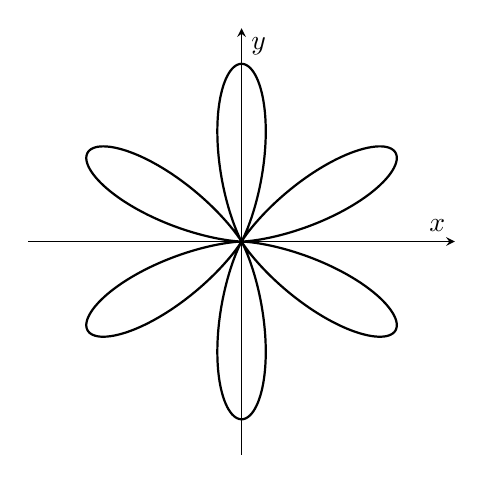
\begin{tikzpicture}
		\begin{axis}[
		  axis lines=middle,
		  xlabel={$x$},
		  ylabel={$y$},
		  width=7cm,
		  height=7cm,
		  xmin=-1.2, xmax=1.2,
		  ymin=-1.2, ymax=1.2,
		  ticks=none,
		  enlargelimits=false,
		  axis equal image
		]
		\addplot[
		  domain=0:360,
		  samples=600,
		  smooth,
		  thick
		]
		({(sin(3*x))^2*cos(x)},{(sin(3*x))^2*sin(x)});
		\end{axis}
		\end{tikzpicture}
	
		Hence the sketch is a 6-petalled rose curve.
	
		\item The polar area formula is
		\[
		A=\frac{1}{2}\int r^2\,\mathrm{d}\theta
		\]
	
		One petal is traced out as $\theta$ goes from $0$ to $\tfrac{\pi}{3}$, since $r=0$ at both endpoints and $r>0$ between them.
	
		So the area of one petal is
		\[
		A_1=\frac{1}{2}\int_0^{\pi/3} a^2\sin^4(3\theta)\,\mathrm{d}\theta
		\]
	
		Use
		\[
		\sin^4 x=\left(\frac{1-\cos 2x}{2}\right)^2
		=\frac{1-2\cos 2x+\cos^2 2x}{4}
		=\frac{1-2\cos 2x+\frac{1+\cos 4x}{2}}{4}
		=\frac{3-4\cos 2x+\cos 4x}{8}
		\]
	
		Therefore
		\[
		\sin^4(3\theta)=\frac{3-4\cos 6\theta+\cos 12\theta}{8}
		\]
	
		Substitute into the integral:
		\begin{align*}
		A_1
		&=\frac{a^2}{2}\int_0^{\pi/3}\frac{3-4\cos 6\theta+\cos 12\theta}{8}\,\mathrm{d}\theta\\
		&=\frac{a^2}{16}\int_0^{\pi/3}\left(3-4\cos 6\theta+\cos 12\theta\right)\,\mathrm{d}\theta\\
		&=\frac{a^2}{16}\left[3\theta-\frac{4}{6}\sin 6\theta+\frac{1}{12}\sin 12\theta\right]_0^{\pi/3}
		\end{align*}
	
		Now evaluate:
		\[
		\sin\left(6\cdot \frac{\pi}{3}\right)=\sin 2\pi=0,
		\qquad
		\sin\left(12\cdot \frac{\pi}{3}\right)=\sin 4\pi=0
		\]
	
		Hence
		\begin{align*}
		A_1
		&=\frac{a^2}{16}\left[3\cdot \frac{\pi}{3}-0+0\right]\\
		&=\frac{\pi a^2}{16}
		\end{align*}
	
		There are 6 identical petals, so the total area is
		\begin{align*}
		A_{\text{total}}
		&=6\cdot \frac{\pi a^2}{16}\\
		&=\frac{3\pi a^2}{8}
		\end{align*}
	
		Therefore the total area enclosed by the curve is
		\[
		\frac{3\pi a^2}{8}
		\]
	  \end{enumerate}
	\end{enumerate}
	\end{tcolorbox}
	
	
	\newpage
	
% ---- Question 3 ----
\questionitem
% [Source: _QBT__Integration_of_Polar_Curves, Q3]

\begin{figure}[H]
    \centering
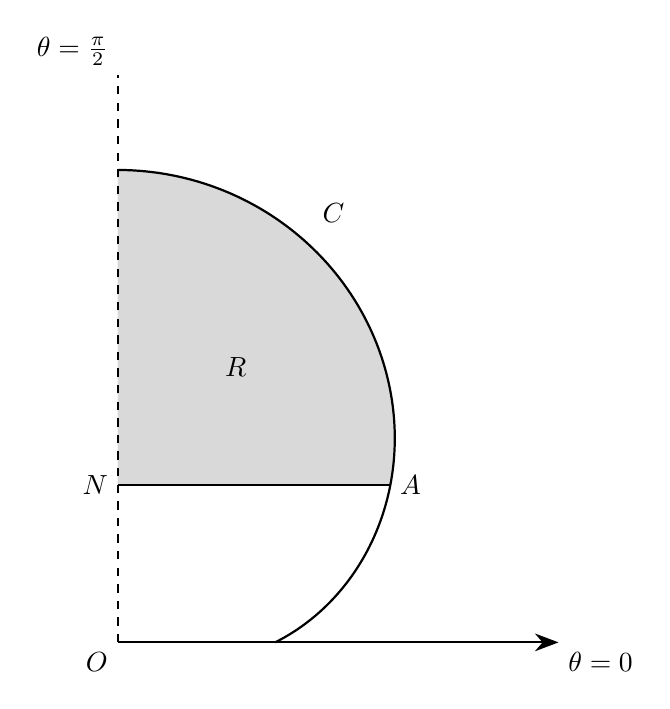
\begin{tikzpicture}[scale=2]
\def\thmax{1.570796}
\def\thA{0.523599}

\coordinate (O) at (0,0);
\coordinate (X) at (2.8,0);
\coordinate (V) at (0,3.6);
\coordinate (A) at (30:2);
\coordinate (N) at ($(O)!(A)!(V)$);
\coordinate (P) at (90:3);

\fill[gray!30] (N) -- (P) --
  plot[smooth, samples=150, domain=\thmax:\thA]
    ({(1+2*sin(deg(\x)))*cos(deg(\x))},{(1+2*sin(deg(\x)))*sin(deg(\x))})
  -- cycle;

\draw[-{Stealth[length=3mm]}, thick] (O) -- (X);
\draw[dashed, thick] (O) -- (V);

\draw[thick]
  plot[smooth, samples=200, domain=0:\thmax]
    ({(1+2*sin(deg(\x)))*cos(deg(\x))},{(1+2*sin(deg(\x)))*sin(deg(\x))});

\draw[thick] (A) -- (N);

\node[below left] at (O) {$O$};
\node[right] at (A) {$A$};
\node[left] at (N) {$N$};
\node[above left] at ({1.1*(1+2*sin(60))*cos(60)},{1.1*(1+2*sin(60))*sin(60)}) {$C$};
\node at (0.75,1.75) {$R$};
\node[above left] at (V) {$\theta=\frac{\pi}{2}$};
\node[below right] at (X) {$\theta=0$};
\end{tikzpicture}
\end{figure}


The curve $C$ shown in the diagram above has polar equation
\[
r=1+2\sin\theta,\quad 0\leq\theta\leq\frac{\pi}{2}
\] \\
The point $A$ on $C$ has $y$-coordinate $1$. \\

The point $N$ lies on the line $\theta=\frac{\pi}{2}$ and $AN$ is perpendicular to the line $\theta=\frac{\pi}{2}$. \\

The finite region $R$, shown shaded in the diagram above, is bounded by the curve $C$, the line $\theta=\frac{\pi}{2}$ and the line $AN$. \\

Find the exact area of the shaded region $R$. \marks{9} \\

	\vspace*{10pt}
	
	\begin{tcolorbox}[colback=white, colframe=scarlet, title={\textbf{Solution}}, breakable, grow to left by=6mm, grow to right by=10mm]
	For the curve
	\[
	r=1+2\sin\theta, \qquad 0\leq \theta \leq \frac{\pi}{2}
	\]
	the point $A$ has $y$-coordinate $1$.
	
	In polar coordinates,
	\[
	y=r\sin\theta
	\]
	so at $A$,
	\[
	(1+2\sin\theta)\sin\theta=1
	\]
	Hence
	\begin{align*}
	2\sin^2\theta+\sin\theta-1&=0\\
	(2\sin\theta-1)(\sin\theta+1)&=0
	\end{align*}
	Since $0\leq \theta \leq \frac{\pi}{2}$, we take
	\[
	\sin\theta=\frac12
	\]
	so
	\[
	\theta_A=\frac{\pi}{6}
	\]
	Then
	\[
	r_A=1+2\sin\frac{\pi}{6}=1+2\left(\frac12\right)=2
	\]
	Therefore
	\[
	A=\left(2,\frac{\pi}{6}\right)
	\]
	and in Cartesian coordinates
	\[
	x=2\cos\frac{\pi}{6}=\sqrt{3}, \qquad y=2\sin\frac{\pi}{6}=1
	\]
	so
	\[
	A=(\sqrt{3},1)
	\]
	
	The line $\theta=\frac{\pi}{2}$ is the $y$-axis, so the line $AN$, perpendicular to it, is horizontal. Since it passes through $A$, its equation is
	\[
	y=1
	\]
	
	Now consider the shaded region $R$. For angles
	\[
	\frac{\pi}{6}\leq \theta \leq \frac{\pi}{2}
	\]
	the outer boundary is the curve
	\[
	r=1+2\sin\theta
	\]
	and the inner boundary is the line $y=1$.
	
	Using $y=r\sin\theta$, the line $y=1$ becomes
	\[
	r\sin\theta=1
	\]
	so
	\[
	r=\frac{1}{\sin\theta}=\operatorname{cosec}\theta
	\]
	
	Using the polar area formula,
	\[
	\text{Area}(R)=\frac12\int_{\pi/6}^{\pi/2}\left[\bigl(1+2\sin\theta\bigr)^2-\operatorname{cosec}^2\theta\right]\mathrm{d}\theta
	\]
	Expand the bracket:
	\begin{align*}
	\text{Area}(R)
	&=\frac12\int_{\pi/6}^{\pi/2}\left(1+4\sin\theta+4\sin^2\theta-\operatorname{cosec}^2\theta\right)\mathrm{d}\theta
	\end{align*}
	
	Now integrate term by term. Using
	\[
	\sin^2\theta=\frac{1-\cos 2\theta}{2}
	\]
	we get
	\begin{align*}
	\int \left(1+4\sin\theta+4\sin^2\theta-\operatorname{cosec}^2\theta\right)\mathrm{d}\theta
	&=\int \left(1+4\sin\theta+2-2\cos2\theta-\operatorname{cosec}^2\theta\right)\mathrm{d}\theta\\
	&=3\theta-4\cos\theta-\sin2\theta+\cot\theta
	\end{align*}
	So
	\[
	\text{Area}(R)=\frac12\left[3\theta-4\cos\theta-\sin2\theta+\cot\theta\right]_{\pi/6}^{\pi/2}
	\]
	
	Now substitute the limits.
	
	At $\theta=\frac{\pi}{2}$:
	\[
	3\left(\frac{\pi}{2}\right)-4\cos\frac{\pi}{2}-\sin\pi+\cot\frac{\pi}{2}
	=\frac{3\pi}{2}
	\]
	
	At $\theta=\frac{\pi}{6}$:
	\begin{align*}
	3\left(\frac{\pi}{6}\right)-4\cos\frac{\pi}{6}-\sin\frac{\pi}{3}+\cot\frac{\pi}{6}
	&=\frac{\pi}{2}-4\left(\frac{\sqrt3}{2}\right)-\frac{\sqrt3}{2}+\sqrt3\\
	&=\frac{\pi}{2}-2\sqrt3-\frac{\sqrt3}{2}+\sqrt3\\
	&=\frac{\pi}{2}-\frac{3\sqrt3}{2}
	\end{align*}
	
	Therefore
	\begin{align*}
	\text{Area}(R)
	&=\frac12\left(\frac{3\pi}{2}-\left(\frac{\pi}{2}-\frac{3\sqrt3}{2}\right)\right)\\
	&=\frac12\left(\pi+\frac{3\sqrt3}{2}\right)\\
	&=\frac{\pi}{2}+\frac{3\sqrt3}{4}
	\end{align*}
	
	Hence the exact area of the shaded region is
	\[
	\frac{\pi}{2}+\frac{3\sqrt3}{4}
	\]
	\end{tcolorbox}
	
	
	\newpage
	
% ---- Question 4 ----
\questionitem
% [Source: _QBT__Integration_of_Polar_Curves, Q4]

The curve $C$ has polar equation
\[
r^2=\frac{\pi^2-(\theta-\pi)^2}{1+(\theta-\pi)^2}\qquad 0\leq\theta\leq2\pi
\] \\
\begin{enumerate}[label=\textbf{(\alph*)}]
  \item Sketch $C$ and state the polar coordinates of the point on $C$ furthest from the pole. \marks{4} \\
  \item Using the substitution $u=\theta-\pi$, or otherwise, find the exact area enclosed by $C$. \marks{6} \\
\end{enumerate}

	\vspace*{10pt}
	
	\begin{tcolorbox}[colback=white, colframe=scarlet, title={\textbf{Solution}}, breakable, grow to left by=6mm, grow to right by=10mm]
	\begin{enumerate}[label=\textbf{(\alph*)}]
	  \item Let
	  \[
	  u=(\theta-\pi)^2
	  \]
	  Then
	  \[
	  r^2=\frac{\pi^2-u}{1+u}, \qquad 0\le u\le \pi^2
	  \]
	  Differentiate with respect to \(u\):
	  \[
	  \frac{\mathrm{d}(r^2)}{\mathrm{d}u}
	  =\frac{-(1+u)-(\pi^2-u)}{(1+u)^2}
	  =-\frac{\pi^2+1}{(1+u)^2}<0
	  \]
	  So \(r^2\) decreases as \(u\) increases, so its maximum occurs when \(u=0\).
	
	  Hence
	  \[
	  (\theta-\pi)^2=0 \implies \theta=\pi
	  \]
	  and then
	  \[
	  r^2=\frac{\pi^2}{1}=\pi^2
	  \]
	  Since we take \(r>0\), this gives
	  \[
	  r=\pi
	  \]
	  So the point on \(C\) furthest from the pole is
	  \[
	  (\pi,\pi)
	  \]
	
	  For the sketch, note that when \(\theta=0\) or \(\theta=2\pi\),
	  \[
	  r^2=\frac{\pi^2-\pi^2}{1+\pi^2}=0
	  \]
	  so the curve passes through the pole.
	
	  Also \(r\) depends only on \((\theta-\pi)^2\), so
	  \[
	  r(2\pi-\theta)=r(\theta)
	  \]
	  Hence the curve is symmetric about the polar axis. Therefore \(C\) is a single closed loop through the pole, with greatest extent on the negative \(x\)-axis.
	
	  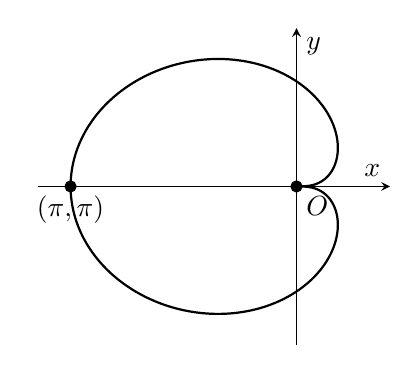
\begin{tikzpicture}
	  \begin{axis}[
		width=0.9\linewidth,
		height=5.6cm,
		axis lines=middle,
		axis equal image,
		xmin=-3.6, xmax=1.3,
		ymin=-2.2, ymax=2.2,
		xlabel={$x$},
		ylabel={$y$},
		xtick=\empty,
		ytick=\empty,
		clip=false
	  ]
	  \addplot[
		thick,
		smooth,
		samples=300,
		domain=0:360,
		variable=\t
	  ]
	  (
		{sqrt((pi^2-((\t*pi/180)-pi)^2)/(1+((\t*pi/180)-pi)^2))*cos(\t)},
		{sqrt((pi^2-((\t*pi/180)-pi)^2)/(1+((\t*pi/180)-pi)^2))*sin(\t)}
	  );
	  \addplot[only marks, mark=*] coordinates {(0,0) (-3.14159,0)};
	  \node[below right] at (axis cs:0,0) {$O$};
	  \node[below] at (axis cs:-3.14159,0) {$(\pi,\pi)$};
	  \end{axis}
	  \end{tikzpicture}
	
	  \item The area enclosed by a polar curve is
	  \[
	  A=\frac12\int_{\alpha}^{\beta} r^2\,\mathrm{d}\theta
	  \]
	  So here
	  \[
	  A=\frac12\int_0^{2\pi}\frac{\pi^2-(\theta-\pi)^2}{1+(\theta-\pi)^2}\,\mathrm{d}\theta
	  \]
	
	  Use the substitution
	  \[
	  u=\theta-\pi
	  \]
	  Then \(\mathrm{d}u=\mathrm{d}\theta\), and the limits change as follows:
	  \[
	  \theta=0 \implies u=-\pi, \qquad \theta=2\pi \implies u=\pi
	  \]
	  Hence
	  \[
	  A=\frac12\int_{-\pi}^{\pi}\frac{\pi^2-u^2}{1+u^2}\,\mathrm{d}u
	  \]
	
	  Now simplify the integrand:
	  \begin{align*}
	  \frac{\pi^2-u^2}{1+u^2}
	  &=\frac{-(1+u^2)+(\pi^2+1)}{1+u^2} \\
	  &=-1+\frac{\pi^2+1}{1+u^2}
	  \end{align*}
	
	  Therefore
	  \begin{align*}
	  A
	  &=\frac12\int_{-\pi}^{\pi}\left(-1+\frac{\pi^2+1}{1+u^2}\right)\,\mathrm{d}u \\
	  &=\frac12\left[-u+(\pi^2+1)\arctan u\right]_{-\pi}^{\pi}
	  \end{align*}
	  using
	  \[
	  \int \frac{1}{1+u^2}\,\mathrm{d}u=\arctan u + c
	  \]
	
	  Now substitute the limits:
	  \begin{align*}
	  A
	  &=\frac12\Bigl[\bigl(-\pi+(\pi^2+1)\arctan\pi\bigr)-\bigl(\pi-(\pi^2+1)\arctan\pi\bigr)\Bigr] \\
	  &=\frac12\Bigl[-2\pi+2(\pi^2+1)\arctan\pi\Bigr] \\
	  &=(\pi^2+1)\arctan(\pi)-\pi
	  \end{align*}
	
	  So the exact area enclosed by \(C\) is
	  \[
	  (\pi^2+1)\arctan(\pi)-\pi
	  \]
	\end{enumerate}
	\end{tcolorbox}
	
	
	\newpage
	
% ---- Question 5 ----
\questionitem
% [Source: _QBT__Integration_of_Polar_Curves, Q5]

\begin{figure}[H]
    \centering
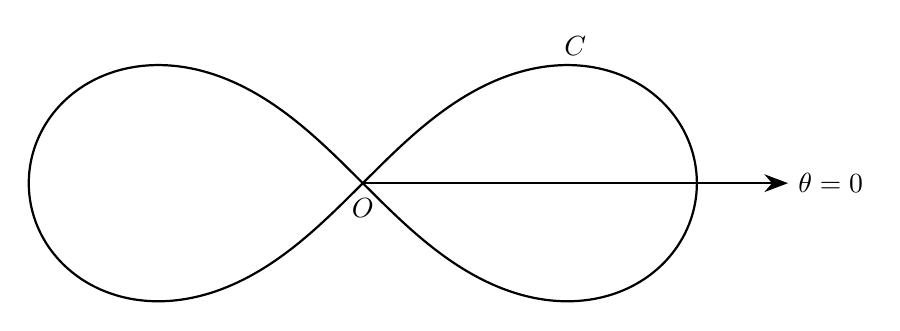
\begin{tikzpicture}[scale=1.5]
\def\K{8}
\def\ArrowLen{3.6}

\coordinate (O) at (0,0);

\draw[-{Stealth[length=3mm]}, thick, black]
  (O) -- (\ArrowLen,0) node[right] {$\theta=0$};

\draw[thick, black]
  (O)
  plot[variable=\t, samples=400, domain=-pi/4:pi/4]
    ({sqrt(max(0,\K*cos(2*\t r)))*cos(\t r)},
     {sqrt(max(0,\K*cos(2*\t r)))*sin(\t r)})
  -- cycle;

\draw[thick, black]
  (O)
  plot[variable=\t, samples=400, domain=3*pi/4:5*pi/4]
    ({sqrt(max(0,\K*cos(2*\t r)))*cos(\t r)},
     {sqrt(max(0,\K*cos(2*\t r)))*sin(\t r)})
  -- cycle;

\node[below, yshift=-2pt] at (O) {$O$};
\node[above right] at
  ({sqrt(\K*cos(2*0.55 r))*cos(0.55 r)},
   {sqrt(\K*cos(2*0.55 r))*sin(0.55 r)})
  {$C$};
\end{tikzpicture}
\end{figure}

\vspace*{10pt}


The diagram below shows the curve $C$ with polar equation $r^2=8\cos 2\theta$. \\

\begin{enumerate}[label=\textbf{(\alph*)}]
  \item Show that a cartesian equation of $C$ is
  \[
  (x^2+y^2)^2=8(x^2-y^2)
  \]
  \marks[-20pt]{4}
  \item Show that the coordinate axes are lines of symmetry of $C$. \marks{2} \\
  \item Find the exact area enclosed by each loop of $C$. \marks{5} \\
\end{enumerate}

	\vspace*{10pt}
	
	\begin{tcolorbox}[colback=white, colframe=scarlet, title={\textbf{Solution}}, breakable, grow to left by=6mm, grow to right by=10mm]
	\begin{enumerate}[label=\textbf{(\alph*)}]
	\item Using
	\[
	x=r\cos\theta,\qquad y=r\sin\theta
	\]
	we have
	\[
	r^2=x^2+y^2
	\]
	Also,
	\[
	\cos 2\theta=\cos^2\theta-\sin^2\theta
	\]
	and since
	\[
	\cos\theta=\frac{x}{r},\qquad \sin\theta=\frac{y}{r}
	\]
	it follows that
	\begin{align*}
	\cos 2\theta
	&=\left(\frac{x}{r}\right)^2-\left(\frac{y}{r}\right)^2 \\
	&=\frac{x^2-y^2}{r^2}
	\end{align*}
	
	Now substitute into the polar equation \(r^2=8\cos 2\theta\):
	\begin{align*}
	r^2&=8\cdot \frac{x^2-y^2}{r^2}
	\end{align*}
	and since \(r^2=x^2+y^2\),
	\begin{align*}
	x^2+y^2&=\frac{8(x^2-y^2)}{x^2+y^2}
	\end{align*}
	Multiplying both sides by \(x^2+y^2\) gives
	\[
	(x^2+y^2)^2=8(x^2-y^2)
	\]
	
	So a cartesian equation of \(C\) is
	\[
	(x^2+y^2)^2=8(x^2-y^2)
	\]
	
	\item To test symmetry in the \(x\)-axis, replace \(y\) by \(-y\):
	\begin{align*}
	(x^2+(-y)^2)^2&=8(x^2-(-y)^2) \\
	(x^2+y^2)^2&=8(x^2-y^2)
	\end{align*}
	which is unchanged, so the curve is symmetric about the \(x\)-axis.
	
	To test symmetry in the \(y\)-axis, replace \(x\) by \(-x\):
	\begin{align*}
	(( -x)^2+y^2)^2&=8(( -x)^2-y^2) \\
	(x^2+y^2)^2&=8(x^2-y^2)
	\end{align*}
	which is also unchanged, so the curve is symmetric about the \(y\)-axis.
	
	Hence the coordinate axes are lines of symmetry of \(C\).
	
	\item For a polar curve, the area enclosed is
	\[
	A=\frac12\int r^2\,\mathrm{d}\theta
	\]
	
	Here
	\[
	r^2=8\cos 2\theta
	\]
	One loop is traced when \(r^2\ge 0\) and \(\theta\) runs from \(-\frac{\pi}{4}\) to \(\frac{\pi}{4}\), since at the endpoints
	\[
	\cos 2\theta=0
	\]
	so the curve passes through the pole.
	
	Therefore the area of one loop is
	\begin{align*}
	A&=\frac12\int_{-\pi/4}^{\pi/4} 8\cos 2\theta \,\mathrm{d}\theta \\
	&=4\int_{-\pi/4}^{\pi/4}\cos 2\theta \,\mathrm{d}\theta \\
	&=4\left[\frac12\sin 2\theta\right]_{-\pi/4}^{\pi/4} \\
	&=2\left[\sin 2\theta\right]_{-\pi/4}^{\pi/4} \\
	&=2\left(\sin\frac{\pi}{2}-\sin\left(-\frac{\pi}{2}\right)\right) \\
	&=2(1-(-1)) \\
	&=4
	\end{align*}
	
	So the exact area enclosed by each loop is
	\[
	4
	\]
	\end{enumerate}
	\end{tcolorbox}
	
	
	\newpage
	
% ---- Question 6 ----
\questionitem
% [Source: _QBT__Integration_of_Polar_Curves, Q6]

\begin{figure}[H]
    \centering
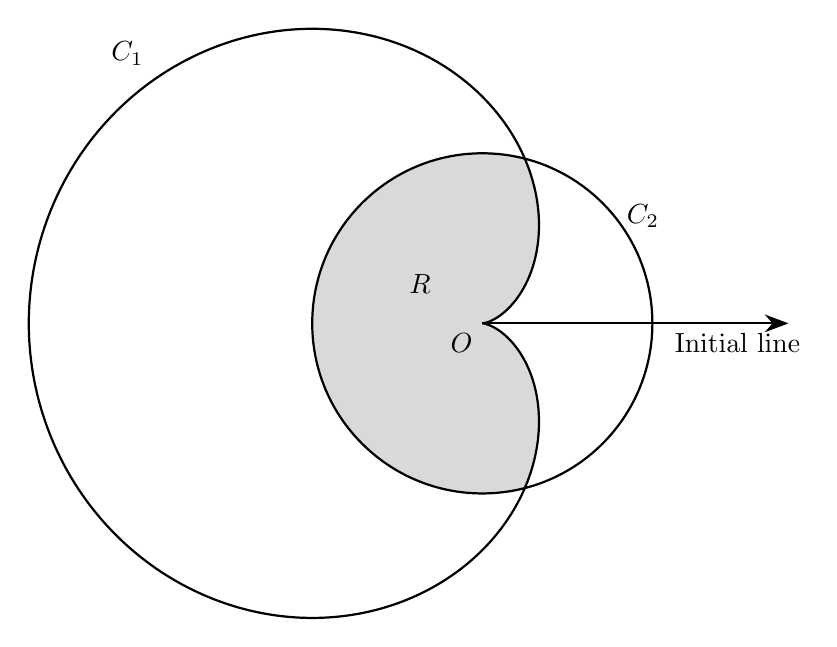
\begin{tikzpicture}[scale=0.9]
\def\aval{1.6}
\def\thA{75.52}
\def\thB{284.48}
\coordinate (O) at (0,0);
\coordinate (COneLabel) at ({2.1*\aval*(1-cos(145))*cos(145)},{2.1*\aval*(1-cos(145))*sin(145)});
\coordinate (CTwoLabel) at (30:1.9*\aval);

\fill[gray!30] (O) --
  plot[smooth, samples=120, domain=0:\thA, variable=\t]
    ({2*\aval*(1-cos(\t))*cos(\t)},{2*\aval*(1-cos(\t))*sin(\t)})
  --
  plot[smooth, samples=180, domain=\thA:\thB, variable=\t]
    ({1.5*\aval*cos(\t)},{1.5*\aval*sin(\t)})
  --
  plot[smooth, samples=120, domain=\thB:360, variable=\t]
    ({2*\aval*(1-cos(\t))*cos(\t)},{2*\aval*(1-cos(\t))*sin(\t)})
  -- cycle;

\draw[thick, black] (O) circle (1.5*\aval);

\draw[thick, black]
  plot[smooth, samples=240, domain=0:360, variable=\t]
    ({2*\aval*(1-cos(\t))*cos(\t)},{2*\aval*(1-cos(\t))*sin(\t)});

\draw[-{Stealth[length=3mm]}, thick, black] (O) -- ({2.7*\aval},0);

\node[below left] at (O) {$O$};
\node[above] at (COneLabel) {$C_1$};
\node[left] at (CTwoLabel) {$C_2$};
\node at ({-0.55*\aval},{0.35*\aval}) {$R$};
\node[below] at ({2.25*\aval},0) {Initial line};
\end{tikzpicture}
\end{figure}


The diagram above shows the curve $C_1$ with polar equation $r=2a(1-\cos\theta)$, $0\leq\theta\leq2\pi$, and the circle $C_2$ with polar equation $r=a$, $0\leq\theta\leq2\pi$, where $a$ is a positive constant. \\
\begin{enumerate}[label=\textbf{(\alph*)}]
  \item Find, in terms of $a$, the polar coordinates of the points where $C_1$ meets $C_2$. \marks{3} \\
\end{enumerate}
The common region enclosed by $C_1$ and $C_2$ is shaded in the diagram above. \\
\begin{enumerate}[label=\textbf{(\alph*)}, resume]
  \item Find the area of the shaded region $R$, giving your answer in the form
  \[
  \frac{1}{12}a^2\left(p\pi+q\sqrt{3}\right)
  \]
  where $p$ and $q$ are integers to be found. \marks{7} \\
\end{enumerate}

	\vspace*{10pt}
	
	\begin{tcolorbox}[colback=white, colframe=scarlet, title={\textbf{Solution}}, breakable, grow to left by=6mm, grow to right by=10mm]
	\begin{enumerate}[label=\textbf{(\alph*)}]
	  \item At the points of intersection, the two values of $r$ are equal, so
	\[
	2a(1-\cos\theta)=a
	\]
	Since $a>0$, divide through by $a$:
	\[
	2(1-\cos\theta)=1
	\]
	\[
	2-2\cos\theta=1
	\]
	\[
	\cos\theta=\frac12
	\]
	For $0\le \theta\le 2\pi$, this gives
	\[
	\theta=\frac{\pi}{3},\ \frac{5\pi}{3}
	\]
	Substituting into either curve gives
	\[
	r=a
	\]
	So the points where $C_1$ meets $C_2$ are
	\[
	(a,\tfrac{\pi}{3}) \quad \text{and} \quad (a,\tfrac{5\pi}{3})
	\]
	  \item For the common region, the boundary is given by the smaller of the two radii.
	
	Compare the curves:
	\[
	2a(1-\cos\theta)\le a
	\]
	\[
	2(1-\cos\theta)\le 1
	\]
	\[
	\cos\theta\ge \frac12
	\]
	So:
	\[
	0\le \theta\le \frac{\pi}{3}
	\quad \text{and} \quad
	\frac{5\pi}{3}\le \theta\le 2\pi
	\]
	give the cardioid $r=2a(1-\cos\theta)$ as the inner curve, and
	\[
	\frac{\pi}{3}\le \theta\le \frac{5\pi}{3}
	\]
	gives the circle $r=a$ as the inner curve.
	
	Using the polar area formula
	\[
	A=\frac12\int r^2\,\mathrm{d}\theta
	\]
	the shaded area is
	\begin{align*}
	A&=\frac12\left[
	\int_0^{\pi/3}\bigl(2a(1-\cos\theta)\bigr)^2\,\mathrm{d}\theta
	+\int_{\pi/3}^{5\pi/3}a^2\,\mathrm{d}\theta
	+\int_{5\pi/3}^{2\pi}\bigl(2a(1-\cos\theta)\bigr)^2\,\mathrm{d}\theta
	\right]
	\end{align*}
	
	By symmetry, the first and third integrals are equal, so
	\begin{align*}
	A&=\int_0^{\pi/3}\bigl(2a(1-\cos\theta)\bigr)^2\,\mathrm{d}\theta
	+\frac12\int_{\pi/3}^{5\pi/3}a^2\,\mathrm{d}\theta \\
	&=4a^2\int_0^{\pi/3}(1-2\cos\theta+\cos^2\theta)\,\mathrm{d}\theta
	+\frac12a^2\left(\frac{5\pi}{3}-\frac{\pi}{3}\right)
	\end{align*}
	
	Now use
	\[
	\cos^2\theta=\frac{1+\cos2\theta}{2}
	\]
	So
	\begin{align*}
	A&=4a^2\int_0^{\pi/3}\left(1-2\cos\theta+\frac{1+\cos2\theta}{2}\right)\,\mathrm{d}\theta
	+\frac12a^2\cdot\frac{4\pi}{3} \\
	&=4a^2\int_0^{\pi/3}\left(\frac32-2\cos\theta+\frac12\cos2\theta\right)\,\mathrm{d}\theta
	+\frac{2\pi a^2}{3}
	\end{align*}
	
	Integrating,
	\begin{align*}
	A&=4a^2\left[\frac32\theta-2\sin\theta+\frac14\sin2\theta\right]_0^{\pi/3}
	+\frac{2\pi a^2}{3} \\
	&=4a^2\left(\frac32\cdot\frac{\pi}{3}-2\sin\frac{\pi}{3}+\frac14\sin\frac{2\pi}{3}\right)
	+\frac{2\pi a^2}{3} \\
	&=4a^2\left(\frac{\pi}{2}-2\cdot\frac{\sqrt3}{2}+\frac14\cdot\frac{\sqrt3}{2}\right)
	+\frac{2\pi a^2}{3} \\
	&=4a^2\left(\frac{\pi}{2}-\sqrt3+\frac{\sqrt3}{8}\right)
	+\frac{2\pi a^2}{3} \\
	&=4a^2\left(\frac{\pi}{2}-\frac{7\sqrt3}{8}\right)
	+\frac{2\pi a^2}{3} \\
	&=2\pi a^2-\frac{7\sqrt3}{2}a^2+\frac{2\pi a^2}{3} \\
	&=\frac{8\pi a^2}{3}-\frac{7\sqrt3\,a^2}{2}
	\end{align*}
	
	Putting this over a denominator of $12$,
	\[
	A=\frac{1}{12}a^2(32\pi-42\sqrt3)
	\]
	
	Hence the shaded area is
	\[
	\frac{1}{12}a^2(32\pi-42\sqrt3)
	\]
	so
	\[
	p=32,\qquad q=-42
	\]
	\end{enumerate}
	\end{tcolorbox}
	
	
	\newpage
	
% ---- Question 7 ----
\questionitem
% [Source: _QBT__Integration_of_Polar_Curves, Q7]

\begin{figure}[H]
    \centering
\begin{tikzpicture}[scale=1.5]
\def\ascl{1}
\coordinate (O) at (0,0);
\coordinate (X) at ({4.6*\ascl},0);
\coordinate (Q) at (45:{4.6*\ascl});
\coordinate (R) at (225:{4.6*\ascl});
\coordinate (A) at (45:{3*\ascl});
\coordinate (B) at ({2*\ascl},0);

\draw[-{Stealth[length=3mm]}, thick] (O) -- (X) node[right] {$\theta=0$};
\draw[dashed] (R) -- (Q);
\pic["$\frac{\pi}{4}$", draw, angle radius=8mm, angle eccentricity=1.35] {angle=X--O--Q};

\draw[thick] (O) circle ({2*\ascl});
\draw[thick, black, samples=400, domain=-180:180, variable=\t]
  plot ({\ascl*(2+sin(2*\t))*cos(\t)},{\ascl*(2+sin(2*\t))*sin(\t)});

\node[below] at (O) {$O$};
\node[right, xshift=3pt] at (A) {$A$};
\node[below right] at (B) {$B$};
\end{tikzpicture}
\end{figure}


The diagram above shows the curve $C$ with polar equation $r=a(2+\sin 2\theta)$ and the circle $r=2a$ for $-\pi\leq\theta\leq\pi$, where $a$ is a positive constant. \\
\begin{enumerate}[label=\textbf{(\alph*)}]
  \item Write down the polar coordinates of the points $A$ and $B$. \marks{2} \\
  \item Explain why $C$ is symmetrical about the line $\theta=\frac{\pi}{4}$. \marks{2} \\
  \item Find, in terms of $a$, the exact total area of the regions that lie inside $C$ and outside the circle. \marks{5} \\
\end{enumerate}

	\vspace*{10pt}
	
	\begin{tcolorbox}[colback=white, colframe=scarlet, title={\textbf{Solution}}, breakable, grow to left by=6mm, grow to right by=10mm]
	\begin{enumerate}[label=\textbf{(\alph*)}]
	  \item For point $A$, the diagram shows $\theta=\dfrac{\pi}{4}$. Then
	  \[
	  r=a\left(2+\sin\frac{\pi}{2}\right)=a(2+1)=3a
	  \]
	  so
	  \[
	  A=\left(3a,\frac{\pi}{4}\right)
	  \]
	
	  For point $B$, $\theta=0$, so
	  \[
	  r=a(2+\sin 0)=2a
	  \]
	  hence
	  \[
	  B=(2a,0)
	  \]
	
	  \item A curve is symmetrical about the line $\theta=\dfrac{\pi}{4}$ if replacing $\theta$ by
	  \[
	  \frac{\pi}{2}-\theta
	  \]
	  leaves the equation unchanged, since reflection in the line $\theta=\dfrac{\pi}{4}$ sends $\theta$ to $\dfrac{\pi}{2}-\theta$.
	
	  Here,
	  \[
	  r=a\left(2+\sin 2\left(\frac{\pi}{2}-\theta\right)\right)
	  =a\left(2+\sin(\pi-2\theta)\right)
	  \]
	  and since $\sin(\pi-2\theta)=\sin 2\theta$,
	  \[
	  r=a(2+\sin 2\theta)
	  \]
	
	  So the equation is unchanged, and therefore $C$ is symmetrical about the line $\theta=\dfrac{\pi}{4}$.
	
	  \item The region is inside $C$ and outside the circle $r=2a$, so we need
	  \[
	  a(2+\sin 2\theta)\ge 2a
	  \]
	  Since $a>0$, this gives
	  \[
	  2+\sin 2\theta \ge 2
	  \]
	  \[
	  \sin 2\theta \ge 0
	  \]
	
	  On $-\pi\le \theta \le \pi$, this happens on
	  \[
	  -\pi\le \theta \le -\frac{\pi}{2}
	  \qquad \text{and} \qquad
	  0\le \theta \le \frac{\pi}{2}
	  \]
	  so there are two equal regions.
	
	  Find the area of one region, for $0\le \theta \le \dfrac{\pi}{2}$.
	
	  Using the polar area formula,
	  \[
	  \text{Area}=\frac12\int r^2\,\mathrm{d}\theta
	  \]
	  the required area for one region is
	  \[
	  A_1=\frac12\int_0^{\pi/2}\left(a^2(2+\sin 2\theta)^2-(2a)^2\right)\,\mathrm{d}\theta
	  \]
	  \[
	  A_1=\frac{a^2}{2}\int_0^{\pi/2}\left((2+\sin 2\theta)^2-4\right)\,\mathrm{d}\theta
	  \]
	
	  Expand the bracket:
	  \[
	  (2+\sin 2\theta)^2-4
	  =4+4\sin 2\theta+\sin^2 2\theta-4
	  =4\sin 2\theta+\sin^2 2\theta
	  \]
	
	  So
	  \[
	  A_1=\frac{a^2}{2}\int_0^{\pi/2}\left(4\sin 2\theta+\sin^2 2\theta\right)\,\mathrm{d}\theta
	  \]
	
	  Now evaluate each part:
	  \[
	  \int_0^{\pi/2}4\sin 2\theta\,\mathrm{d}\theta
	  =\left[-2\cos 2\theta\right]_0^{\pi/2}
	  =2-(-2)=4
	  \]
	
	  Also,
	  \[
	  \sin^2 2\theta=\frac{1-\cos 4\theta}{2}
	  \]
	  so
	  \[
	  \int_0^{\pi/2}\sin^2 2\theta\,\mathrm{d}\theta
	  =\int_0^{\pi/2}\frac{1-\cos 4\theta}{2}\,\mathrm{d}\theta
	  =\left[\frac{\theta}{2}-\frac{\sin 4\theta}{8}\right]_0^{\pi/2}
	  =\frac{\pi}{4}
	  \]
	
	  Therefore
	  \[
	  A_1=\frac{a^2}{2}\left(4+\frac{\pi}{4}\right)
	  =a^2\left(2+\frac{\pi}{8}\right)
	  \]
	
	  There are two such regions, so the total area is
	  \[
	  2A_1=2a^2\left(2+\frac{\pi}{8}\right)
	  =a^2\left(4+\frac{\pi}{4}\right)
	  =\frac{a^2(16+\pi)}{4}
	  \]
	
	  Hence the exact total area is
	  \[
	  \frac{a^2(16+\pi)}{4}
	  \]
	\end{enumerate}
	\end{tcolorbox}
	
	
	\newpage
	
% ---- Question 8 ----
\questionitem
% [Source: _QBT__Integration_of_Polar_Curves, Q8]

\begin{figure}[H]
    \centering
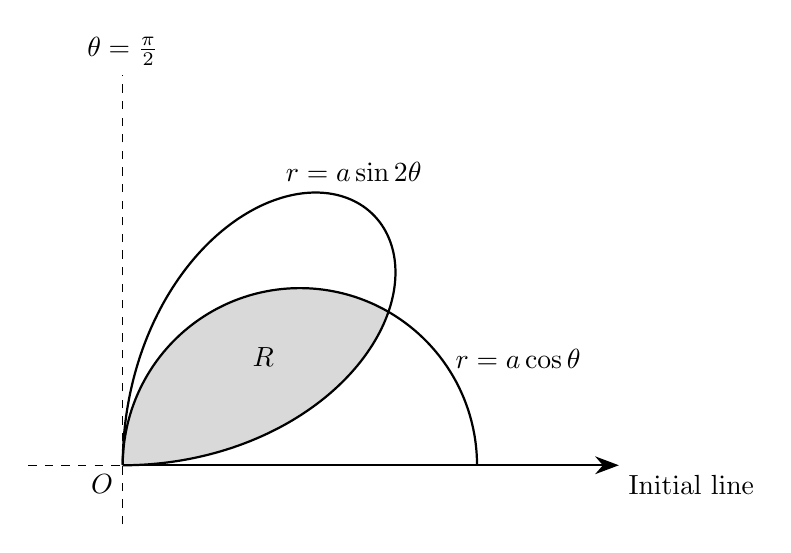
\begin{tikzpicture}[scale=1.5]
\def\a{3}
\pgfmathsetmacro{\thI}{pi/6}
\pgfmathsetmacro{\thMax}{pi/2}
\coordinate (O) at (0,0);
\coordinate (Xleft) at (-0.8,0);
\coordinate (Xend) at (4.2,0);
\coordinate (Ybot) at (0,-0.5);
\coordinate (Ytop) at (0,3.3);

\draw[dashed] (Xleft) -- (O);
\draw[-{Stealth[length=3mm]}, thick] (O) -- (Xend);
\draw[dashed] (Ybot) -- (Ytop);

\fill[gray!30]
  (O) --
  plot[smooth, samples=120, domain=0:\thI, variable=\t]
    ({\a*sin(2*deg(\t))*cos(deg(\t))},{\a*sin(2*deg(\t))*sin(deg(\t))})
  --
  plot[smooth, samples=120, domain=\thI:\thMax, variable=\t]
    ({\a*cos(deg(\t))*cos(deg(\t))},{\a*cos(deg(\t))*sin(deg(\t))})
  -- cycle;

\draw[thick, black]
  plot[smooth, samples=200, domain=0:\thMax, variable=\t]
    ({\a*sin(2*deg(\t))*cos(deg(\t))},{\a*sin(2*deg(\t))*sin(deg(\t))});

\draw[thick, black]
  plot[smooth, samples=200, domain=0:\thMax, variable=\t]
    ({\a*cos(deg(\t))*cos(deg(\t))},{\a*cos(deg(\t))*sin(deg(\t))});

\pgfmathsetmacro{\rR}{0.5*\a}
\coordinate (Rlab) at (37.5:\rR);
\pgfmathsetmacro{\thLabelRose}{pi/3}
\coordinate (Lrose) at ({\a*sin(2*deg(\thLabelRose))*cos(deg(\thLabelRose))},{\a*sin(2*deg(\thLabelRose))*sin(deg(\thLabelRose))});
\pgfmathsetmacro{\thLabelCircle}{pi/8}
\coordinate (Lcircle) at ({\a*cos(deg(\thLabelCircle))*cos(deg(\thLabelCircle))},{\a*cos(deg(\thLabelCircle))*sin(deg(\thLabelCircle))});

\node[below left] at (O) {$O$};
\node[below right] at (Xend) {Initial line};
\node[above] at (Ytop) {$\theta=\frac{\pi}{2}$};
\node at (Rlab) {$R$};
\node[above right, yshift=3pt] at (Lrose) {$r=a\sin 2\theta$};
\node[below right, xshift=7.5pt] at (Lcircle) {$r=a\cos\theta$};
\end{tikzpicture}
\end{figure}


In the first quadrant, the curve $r=a\sin 2\theta$ intersects the circle $r=a\cos\theta$ at the pole and at one other point. \\

The region $R$ shown consists of the points that lie inside both curves. \\

Find the exact area of $R$ in terms of $a$. \marks{8} \\

	\vspace*{10pt}
	
	\begin{tcolorbox}[colback=white, colframe=scarlet, title={\textbf{Solution}}, breakable, grow to left by=6mm, grow to right by=10mm]
	For the points of intersection, set the two expressions for \(r\) equal:
	\[
	a\sin 2\theta=a\cos\theta
	\]
	
	Since \(a\neq 0\),
	\[
	\sin 2\theta=\cos\theta
	\]
	
	Using \(\sin 2\theta=2\sin\theta\cos\theta\),
	\[
	2\sin\theta\cos\theta=\cos\theta
	\]
	\[
	\cos\theta(2\sin\theta-1)=0
	\]
	
	In the first quadrant, \(0\le \theta\le \frac{\pi}{2}\), so
	\[
	\cos\theta=0 \Rightarrow \theta=\frac{\pi}{2}
	\]
	or
	\[
	2\sin\theta-1=0 \Rightarrow \sin\theta=\frac12 \Rightarrow \theta=\frac{\pi}{6}
	\]
	
	At \(\theta=\frac{\pi}{2}\),
	\[
	r=a\cos\frac{\pi}{2}=0
	\]
	so this is the pole.
	
	At the other intersection,
	\[
	r=a\cos\frac{\pi}{6}=\frac{a\sqrt3}{2}
	\]
	
	So the non-pole intersection is at
	\[
	\left(r,\theta\right)=\left(\frac{a\sqrt3}{2},\frac{\pi}{6}\right)
	\]
	
	Now find which curve forms the boundary of the region inside both curves.
	
	For \(0\le \theta\le \frac{\pi}{6}\),
	\[
	a\sin2\theta \le a\cos\theta
	\]
	so the smaller radius is \(r=a\sin2\theta\).
	
	For \(\frac{\pi}{6}\le \theta\le \frac{\pi}{2}\),
	\[
	a\cos\theta \le a\sin2\theta
	\]
	so the smaller radius is \(r=a\cos\theta\).
	
	Hence, using the polar area formula
	\[
	\text{Area}=\frac12\int r^2\,\mathrm{d}\theta
	\]
	the required area is
	\[
	\text{Area}(R)=\frac12a^2\left(\int_0^{\pi/6}\sin^22\theta\,\mathrm{d}\theta+\int_{\pi/6}^{\pi/2}\cos^2\theta\,\mathrm{d}\theta\right)
	\]
	
	Now evaluate the integrals.
	
	First, use
	\[
	\sin^22\theta=\frac{1-\cos4\theta}{2}
	\]
	Then
	\begin{align*}
	\int_0^{\pi/6}\sin^22\theta\,\mathrm{d}\theta
	&=\int_0^{\pi/6}\frac{1-\cos4\theta}{2}\,\mathrm{d}\theta \\
	&=\left[\frac{\theta}{2}-\frac{\sin4\theta}{8}\right]_0^{\pi/6} \\
	&=\frac{\pi}{12}-\frac{\sin(2\pi/3)}{8} \\
	&=\frac{\pi}{12}-\frac{\sqrt3}{16}
	\end{align*}
	
	Next, use
	\[
	\cos^2\theta=\frac{1+\cos2\theta}{2}
	\]
	Then
	\begin{align*}
	\int_{\pi/6}^{\pi/2}\cos^2\theta\,\mathrm{d}\theta
	&=\int_{\pi/6}^{\pi/2}\frac{1+\cos2\theta}{2}\,\mathrm{d}\theta \\
	&=\left[\frac{\theta}{2}+\frac{\sin2\theta}{4}\right]_{\pi/6}^{\pi/2} \\
	&=\left(\frac{\pi}{4}+0\right)-\left(\frac{\pi}{12}+\frac{\sin(\pi/3)}{4}\right) \\
	&=\frac{\pi}{6}-\frac{\sqrt3}{8}
	\end{align*}
	
	Substitute back:
	\begin{align*}
	\text{Area}(R)
	&=\frac12a^2\left(\frac{\pi}{12}-\frac{\sqrt3}{16}+\frac{\pi}{6}-\frac{\sqrt3}{8}\right) \\
	&=\frac12a^2\left(\frac{\pi}{4}-\frac{3\sqrt3}{16}\right) \\
	&=\frac{a^2(4\pi-3\sqrt3)}{32}
	\end{align*}
	
	Hence the exact area of \(R\) is
	\[
	\frac{a^2(4\pi-3\sqrt3)}{32}
	\]
	\end{tcolorbox}
	
	
	\newpage
	
% ---- Question 9 ----
\questionitem
% [Source: _QBT__Integration_of_Polar_Curves, Q9]

\begin{enumerate}[label=\textbf{(\alph*)}]
  \item On the same diagram, sketch the curve $C_1$ with polar equation
  \[
  r=2(1+\cos\theta),\quad 0\leq\theta\leq2\pi
  \]
  and the curve $C_2$ with polar equation $\theta=\frac{2\pi}{3}$. \marks{3} \\
  \item Find the area of the smaller region bounded by $C_1$ and $C_2$. \marks{6} \\
\end{enumerate}

	\vspace*{10pt}
	
	\begin{tcolorbox}[colback=white, colframe=scarlet, title={\textbf{Solution}}, breakable, grow to left by=6mm, grow to right by=10mm]
	\begin{enumerate}[label=\textbf{(\alph*)}]
	  \item For \(C_1\),
	\[
	r=2(1+\cos\theta)
	\]
	Since this depends on \(\cos\theta\), the curve is symmetric about the initial line.
	
	Key values are
	\[
	\theta=0 \implies r=4,\qquad
	\theta=\pi \implies r=0,\qquad
	\theta=\frac{\pi}{2},\frac{3\pi}{2} \implies r=2
	\]
	So \(C_1\) is a cardioid with maximum \(r=4\) on the initial line and a cusp at the pole.
	
	For \(C_2\),
	\[
	\theta=\frac{2\pi}{3}
	\]
	is the ray through the pole making an angle \(120^\circ\) with the initial line.
	
	The other intersection of the two curves is found by substituting \(\theta=\frac{2\pi}{3}\) into \(C_1\):
	\[
	r=2\left(1+\cos\frac{2\pi}{3}\right)=2\left(1-\frac12\right)=1
	\]
	So the curves meet at the pole and at \(r=1,\ \theta=\frac{2\pi}{3}\).
	
	A suitable sketch is: \vspace*{15pt}
	
	\begin{tikzpicture}[scale=1.0]
	\draw[->] (-1.2,0) -- (4.7,0) node[right] {$x$};
	\draw[->] (0,-2.6) -- (0,2.6) node[above] {$y$};
	
	\draw[thick,domain=0:360,samples=300,smooth,variable=\t]
	plot ({2*(1+cos(\t))*cos(\t)},{2*(1+cos(\t))*sin(\t)});
	
	\draw[thick,->] (0,0) -- ++(120:3) node[above left] {$C_2:\ \theta=\frac{2\pi}{3}$};
	
	\fill (0,0) circle (1.2pt);
	\node[below left] at (0,0) {$O$};
	
	\fill (4,0) circle (1.2pt);
	\fill (-0.5,0.8660254) circle (1.2pt);
	
	\node[above] at (2.0,1.65) {$C_1$};
	\end{tikzpicture}
	
	  \item The smaller region is the part inside the cardioid between
	\[
	\theta=\frac{2\pi}{3}\quad \text{and}\quad \theta=\pi
	\]
	
	Using the polar area formula
	\[
	A=\frac12\int_{\alpha}^{\beta} r^2\,\mathrm{d}\theta
	\]
	we get
	\[
	A=\frac12\int_{2\pi/3}^{\pi}\left[2(1+\cos\theta)\right]^2\,\mathrm{d}\theta
	\]
	
	Now simplify the integrand:
	\begin{align*}
	A&=2\int_{2\pi/3}^{\pi}(1+2\cos\theta+\cos^2\theta)\,\mathrm{d}\theta \\
	&=2\int_{2\pi/3}^{\pi}\left(1+2\cos\theta+\frac{1+\cos2\theta}{2}\right)\,\mathrm{d}\theta \\
	&=\int_{2\pi/3}^{\pi}(3+4\cos\theta+\cos2\theta)\,\mathrm{d}\theta
	\end{align*}
	
	Integrating,
	\begin{align*}
	A&=\left[3\theta+4\sin\theta+\frac12\sin2\theta\right]_{2\pi/3}^{\pi} \\
	&=\left(3\pi+4\sin\pi+\frac12\sin2\pi\right)
	-\left(3\cdot\frac{2\pi}{3}+4\sin\frac{2\pi}{3}+\frac12\sin\frac{4\pi}{3}\right) \\
	&=3\pi-\left(2\pi+4\cdot\frac{\sqrt3}{2}+\frac12\cdot\left(-\frac{\sqrt3}{2}\right)\right) \\
	&=\pi-2\sqrt3+\frac{\sqrt3}{4} \\
	&=\pi-\frac{7\sqrt3}{4}
	\end{align*}
	
	So the area of the smaller region is
	\[
	\pi-\frac{7\sqrt3}{4}\approx 0.111
	\]
	  \end{enumerate}
	\end{tcolorbox}
	
	
	\newpage
	
% ---- Question 10 ----
\questionitem
% [Source: _QBT__Integration_of_Polar_Curves, Q10]

\begin{figure}[H]
    \centering
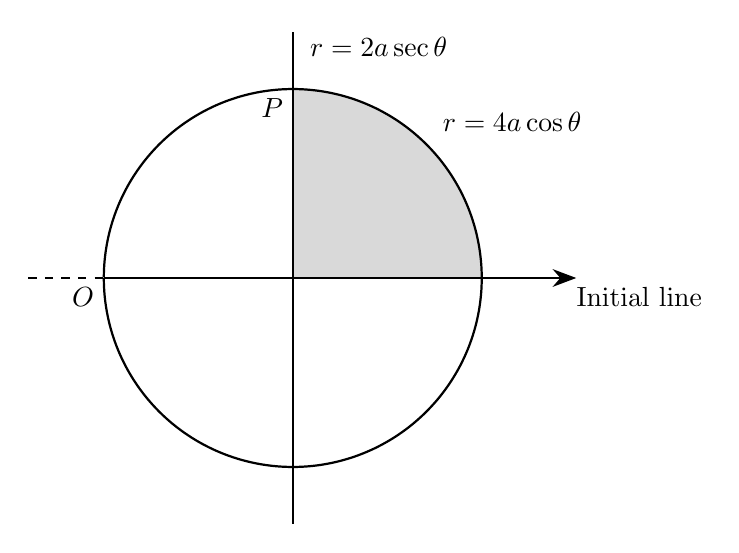
\begin{tikzpicture}[scale=1.2]
\def\a{1}
\def\th{0.785398} % pi/4

\coordinate (O) at (0,0);
\coordinate (A) at ({4*\a},0);
\coordinate (B) at ({2*\a},0);

\path[name path=circle]
  plot[smooth, samples=240, domain=-1.570796:1.570796]
    ({4*\a*cos(deg(\x))*cos(deg(\x))},
     {4*\a*cos(deg(\x))*sin(deg(\x))});
\path[name path=line] ({2*\a},{-2.6*\a}) -- ({2*\a},{2.6*\a});
\path[name intersections={of=circle and line, by={Q,P}}];

\fill[gray!30]
  (B) -- (P) --
  plot[smooth, samples=120, domain=\th:0]
    ({4*\a*cos(deg(\x))*cos(deg(\x))},
     {4*\a*cos(deg(\x))*sin(deg(\x))})
  -- cycle;

\draw[dashed, black] (-0.8,0) -- (0,0);
\draw[-{Stealth[length=3mm]}, thick, black] (0,0) -- (5,0);

\draw[thick, black]
  plot[smooth, samples=240, domain=-1.570796:1.570796]
    ({4*\a*cos(deg(\x))*cos(deg(\x))},
     {4*\a*cos(deg(\x))*sin(deg(\x))});
\draw[thick, black] ({2*\a},{-2.6*\a}) -- ({2*\a},{2.6*\a});

\node[below left] at (O) {$O$};
\node[below left] at (P) {$P$};
\node[below right] at (4.9,0) {Initial line};
\node[right] at ({2.08*\a},{2.45*\a}) {$r = 2a\sec\theta$};
\node[above, xshift=40pt] at ({3.15*\a},{1.45*\a}) {$r = 4a\cos\theta$};
\end{tikzpicture}
\end{figure}


The diagram shows a sketch of the curves with polar equations
\[
r=4a\cos\theta \text{ and } r=2a\sec\theta,\quad a>0
\] \\
\begin{enumerate}[label=\textbf{(\alph*)}]
  \item Find the polar coordinates of the point of intersection $P$ of the two curves in the first quadrant. \marks{4} \\
  \item Find the area, shaded in the figure, bounded by the two curves and by the initial line $\theta=0$, giving your answer in terms of $a$ and $\pi$. \marks{6} \\
\end{enumerate}

	\vspace*{10pt}
	
	\begin{tcolorbox}[colback=white, colframe=scarlet, title={\textbf{Solution}}, breakable, grow to left by=6mm, grow to right by=10mm]
	\begin{enumerate}[label=\textbf{(\alph*)}]
	  \item At a point of intersection, the two expressions for $r$ are equal:
	\[
	4a\cos\theta=2a\sec\theta
	\]
	
	Since $a>0$, divide by $2a$:
	\[
	2\cos\theta=\sec\theta=\frac{1}{\cos\theta}
	\]
	
	So
	\[
	2\cos^2\theta=1
	\]
	\[
	\cos^2\theta=\frac12
	\]
	
	In the first quadrant, $\cos\theta>0$, so
	\[
	\cos\theta=\frac{1}{\sqrt2}
	\]
	hence
	\[
	\theta=\frac{\pi}{4}
	\]
	
	Now find $r$:
	\[
	r=4a\cos\frac{\pi}{4}=4a\cdot \frac{1}{\sqrt2}=2\sqrt2\,a
	\]
	
	So the polar coordinates of $P$ are
	\[
	\boxed{\left(2\sqrt2\,a,\frac{\pi}{4}\right)}
	\]
	
	  \item The required shaded area is between the curves from $\theta=0$ to the intersection at $\theta=\frac{\pi}{4}$.
	
	For $0\le \theta \le \frac{\pi}{4}$, the outer curve is
	\[
	r=4a\cos\theta
	\]
	and the inner curve is
	\[
	r=2a\sec\theta
	\]
	
	So, using
	\[
	\text{Area}=\frac12\int_{\alpha}^{\beta}\left(r_{\text{outer}}^2-r_{\text{inner}}^2\right)\,\mathrm{d}\theta
	\]
	we get
	\[
	A=\frac12\int_0^{\pi/4}\left((4a\cos\theta)^2-(2a\sec\theta)^2\right)\,\mathrm{d}\theta
	\]
	
	Simplify:
	\[
	A=\frac12\int_0^{\pi/4}\left(16a^2\cos^2\theta-4a^2\sec^2\theta\right)\,\mathrm{d}\theta
	\]
	\[
	A=8a^2\int_0^{\pi/4}\cos^2\theta\,\mathrm{d}\theta-2a^2\int_0^{\pi/4}\sec^2\theta\,\mathrm{d}\theta
	\]
	
	Use
	\[
	\cos^2\theta=\frac{1+\cos 2\theta}{2}
	\]
	so
	\[
	\int \cos^2\theta\,\mathrm{d}\theta=\frac{\theta}{2}+\frac{\sin 2\theta}{4}
	\]
	
	Therefore
	\begin{align*}
	A&=8a^2\left[\frac{\theta}{2}+\frac{\sin 2\theta}{4}\right]_0^{\pi/4}
	-2a^2\left[\tan\theta\right]_0^{\pi/4} \\
	&=8a^2\left(\frac{\pi}{8}+\frac14\right)-2a^2(1) \\
	&=\pi a^2+2a^2-2a^2 \\
	&=\pi a^2
	\end{align*}
	
	Hence the shaded area is
	\[
	\boxed{\pi a^2}
	\]
	\end{enumerate}
	\end{tcolorbox}
	
	
	\newpage
	
% ---- Question 11 ----
\questionitem
% [Source: _QBT__Integration_of_Polar_Curves, Q11]

\begin{figure}[H]
    \centering
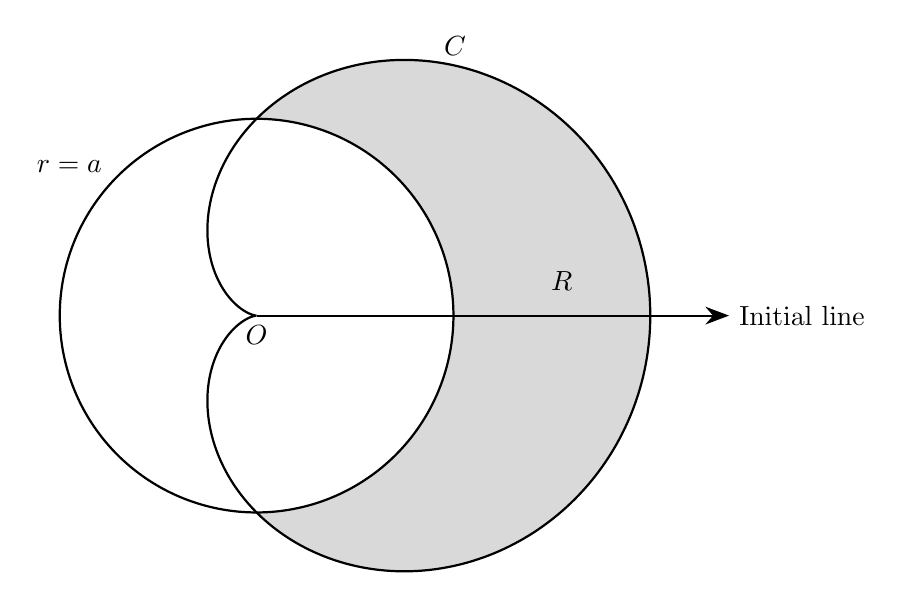
\begin{tikzpicture}[scale=1.25]
\def\a{2}
\coordinate (R) at ({1.55*\a},0.35);

\fill[gray!30]
  plot[smooth, samples=200, domain=-1.570796:1.570796, variable=\t]
    ({(\a*(1+cos(deg(\t))))*cos(deg(\t))},{(\a*(1+cos(deg(\t))))*sin(deg(\t))})
  --
  plot[smooth, samples=200, domain=1.570796:-1.570796, variable=\t]
    ({\a*cos(deg(\t))},{\a*sin(deg(\t))})
  -- cycle;

\pgfmathsetmacro{\tC}{0.9}
\draw[thick, black]
  plot[smooth, samples=300, domain=-pi:pi, variable=\t]
    ({(\a*(1+cos(deg(\t))))*cos(deg(\t))},
     {(\a*(1+cos(deg(\t))))*sin(deg(\t))});
\node[above] at
  ({(\a*(1+cos(deg(\tC))))*cos(deg(\tC))},
   {(\a*(1+cos(deg(\tC))))*sin(deg(\tC))}) {$C$};

\pgfmathsetmacro{\tr}{2.4}
\draw[thick, black]
  plot[smooth, samples=300, domain=0:2*pi, variable=\t]
    ({\a*cos(deg(\t))},
     {\a*sin(deg(\t))});
\node[above left] at
  ({\a*cos(deg(\tr))},
   {\a*sin(deg(\tr))}) {$r=a$};

\draw[-{Stealth[length=3mm]}, thick, black] (0,0) -- (4.8,0) node[right] {Initial line};
\node[below] at (0,0) {$O$};
\node at (R) {$R$};
\end{tikzpicture}
\end{figure}


The figure above shows a sketch of the curve $C$ with polar equation
\[
r=a(1+\cos\theta)
\] \\
and the circle
\[
r=a
\] \\
where $a>0$ and $-\pi\leq\theta\leq\pi$. \\

The shaded region inside $C$ and outside the circle has area
\[
18+\frac{9\pi}{4}
\] \\
Find the value of $a$. \marks{8} \\

	\vspace*{10pt}
	
	\begin{tcolorbox}[colback=white, colframe=scarlet, title={\textbf{Solution}}, breakable, grow to left by=6mm, grow to right by=10mm]
	For the shaded region, we first find where the curve and the circle meet.
	
	The curve is
	\[
	r=a(1+\cos\theta)
	\]
	and the circle is
	\[
	r=a
	\]
	
	At points of intersection,
	\[
	a(1+\cos\theta)=a
	\]
	Since $a>0$, divide by $a$:
	\[
	1+\cos\theta=1
	\]
	so
	\[
	\cos\theta=0
	\]
	Hence
	\[
	\theta=\pm \frac{\pi}{2}
	\]
	
	So the shaded region is between $\theta=-\frac{\pi}{2}$ and $\theta=\frac{\pi}{2}$, with outer radius
	\[
	r=a(1+\cos\theta)
	\]
	and inner radius
	\[
	r=a
	\]
	
	Using the polar area formula,
	\[
	\text{Area}=\frac12\int_{\alpha}^{\beta} r^2\,\mathrm{d}\theta
	\]
	the shaded area is
	\[
	\frac12\int_{-\pi/2}^{\pi/2}\left([a(1+\cos\theta)]^2-a^2\right)\,\mathrm{d}\theta
	\]
	
	Expand the bracket:
	\begin{align*}
	[a(1+\cos\theta)]^2-a^2
	&=a^2(1+2\cos\theta+\cos^2\theta)-a^2 \\
	&=a^2(2\cos\theta+\cos^2\theta)
	\end{align*}
	
	So
	\[
	\text{Area}=\frac{a^2}{2}\int_{-\pi/2}^{\pi/2}\left(2\cos\theta+\cos^2\theta\right)\,\mathrm{d}\theta
	\]
	
	Now evaluate the two parts separately.
	
	First,
	\[
	\int_{-\pi/2}^{\pi/2} 2\cos\theta\,\mathrm{d}\theta
	=2[\sin\theta]_{-\pi/2}^{\pi/2}
	=2(1-(-1))=4
	\]
	
	For the second part, use
	\[
	\cos^2\theta=\frac{1+\cos2\theta}{2}
	\]
	So
	\begin{align*}
	\int_{-\pi/2}^{\pi/2}\cos^2\theta\,\mathrm{d}\theta
	&=\int_{-\pi/2}^{\pi/2}\frac{1+\cos2\theta}{2}\,\mathrm{d}\theta \\
	&=\left[\frac{\theta}{2}+\frac{\sin2\theta}{4}\right]_{-\pi/2}^{\pi/2} \\
	&=\left(\frac{\pi}{4}+0\right)-\left(-\frac{\pi}{4}+0\right) \\
	&=\frac{\pi}{2}
	\end{align*}
	
	Therefore
	\begin{align*}
	\text{Area}
	&=\frac{a^2}{2}\left(4+\frac{\pi}{2}\right) \\
	&=2a^2+\frac{\pi a^2}{4}
	\end{align*}
	
	We are told this area is
	\[
	18+\frac{9\pi}{4}
	\]
	So
	\[
	2a^2+\frac{\pi a^2}{4}=18+\frac{9\pi}{4}
	\]
	
	Multiply through by $4$:
	\[
	8a^2+\pi a^2=72+9\pi
	\]
	\[
	a^2(8+\pi)=9(8+\pi)
	\]
	Hence
	\[
	a^2=9
	\]
	Since $a>0$,
	\[
	a=3
	\]
	
	Therefore, the value of $a$ is $3$.
	\end{tcolorbox}
	
	
	\newpage
	
% ---- Question 12 ----
\questionitem
% [Source: _QBT__Integration_of_Polar_Curves, Q12]

\begin{figure}[H]
    \centering
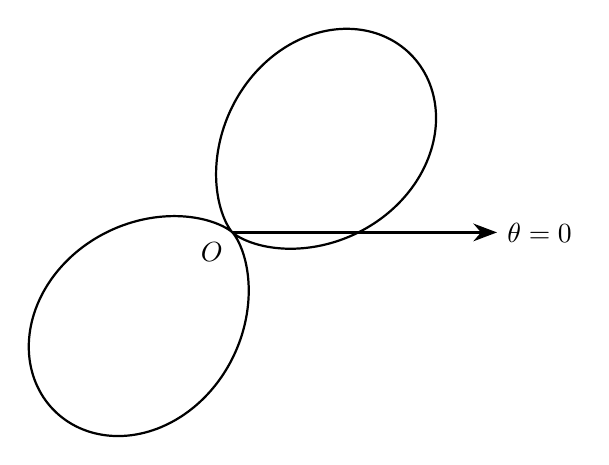
\begin{tikzpicture}[scale=1.6]
\def\twopi{6.283185}
\draw[-{Stealth[length=3mm]}, thick] (0,0) -- (2.1,0) node[right] {$\theta = 0$};
\draw[thick, black]
  plot[smooth, samples=400, domain=0:\twopi]
    ({(1+sin(deg(2*\x)))*cos(deg(\x))},{(1+sin(deg(2*\x)))*sin(deg(\x))});
\node[below left] at (0,0) {$O$};
\end{tikzpicture}
\end{figure}


The diagram below shows the curve with polar equation $r=1+\sin 2\theta$ for $0\leq\theta\leq2\pi$. \\
\begin{enumerate}[label=\textbf{(\alph*)}]
  \item Find the values of $\theta$ at the pole. \marks{1} \\
  \item Find the polar coordinates of the points on the curve where $r$ takes its maximum value. \marks{2} \\
  \item Find the exact total area enclosed by the curve. \marks{4} \\
  \item Find a Cartesian equation for the curve. \marks{2} \\
\end{enumerate}

\vspace*{10pt}
	
\begin{tcolorbox}[colback=white, colframe=scarlet, title={\textbf{Solution}}, breakable, grow to left by=6mm, grow to right by=10mm]
\begin{enumerate}[label=\textbf{(\alph*)}]
	  \item At the pole, \(r=0\). So
	  \[
	  1+\sin 2\theta=0
	  \]
	  \[
	  \sin 2\theta=-1
	  \]
	  For \(0\leq \theta \leq 2\pi\), this gives
	  \[
	  2\theta=\frac{3\pi}{2},\ \frac{7\pi}{2}
	  \]
	  so
	  \[
	  \theta=\frac{3\pi}{4},\ \frac{7\pi}{4}
	  \]
	  Therefore the values of \(\theta\) at the pole are \(\displaystyle \frac{3\pi}{4}\) and \(\displaystyle \frac{7\pi}{4}\).
	
	  \item \(r=1+\sin 2\theta\) is largest when \(\sin 2\theta=1\). Hence
	  \[
	  r_{\max}=1+1=2
	  \]
	  Now \(\sin 2\theta=1\) when
	  \[
	  2\theta=\frac{\pi}{2},\ \frac{5\pi}{2}
	  \]
	  so
	  \[
	  \theta=\frac{\pi}{4},\ \frac{5\pi}{4}
	  \]
	  Therefore the points are
	  \[
	  (2,\tfrac{\pi}{4}) \quad \text{and} \quad (2,\tfrac{5\pi}{4})
	  \]
	
	  \item The total area enclosed by a polar curve is
	  \[
	  A=\frac12\int_0^{2\pi} r^2\,\mathrm{d}\theta
	  \]
	  So here
	  \[
	  A=\frac12\int_0^{2\pi}(1+\sin 2\theta)^2\,\mathrm{d}\theta
	  \]
	  Expanding,
	  \[
	  A=\frac12\int_0^{2\pi}\left(1+2\sin 2\theta+\sin^2 2\theta\right)\,\mathrm{d}\theta
	  \]
	  Using
	  \[
	  \sin^2 2\theta=\frac{1-\cos 4\theta}{2}
	  \]
	  gives
	  \begin{align*}
	  A&=\frac12\int_0^{2\pi}\left(1+2\sin 2\theta+\frac{1-\cos 4\theta}{2}\right)\,\mathrm{d}\theta \\
	   &=\frac12\int_0^{2\pi}\left(\frac32+2\sin 2\theta-\frac12\cos 4\theta\right)\,\mathrm{d}\theta
	  \end{align*}
	  Integrating term by term,
	  \begin{align*}
	  A&=\frac12\left[\frac32\theta-\cos 2\theta-\frac18\sin 4\theta\right]_0^{2\pi} \\
	   &=\frac12\left(3\pi-1-0-(-1)\right) \\
	   &=\frac12(3\pi)
	  \end{align*}
	  Hence the exact total area enclosed is
	  \[
	  \frac{3\pi}{2}
	  \]
	
	  \item Using
	  \[
	  x=r\cos\theta,\qquad y=r\sin\theta,\qquad r^2=x^2+y^2
	  \]
	  and \(\sin 2\theta=2\sin\theta\cos\theta\),
	  \[
	  r=1+2\sin\theta\cos\theta
	  \]
	  Now
	  \[
	  \sin\theta=\frac{y}{r},\qquad \cos\theta=\frac{x}{r}
	  \]
	  so
	  \[
	  r=1+\frac{2xy}{r^2}
	  \]
	  Multiplying by \(r^2\),
	  \[
	  r^3=r^2+2xy
	  \]
	  Since \(r^2=x^2+y^2\),
	  \[
	  r^3=x^2+y^2+2xy=(x+y)^2
	  \]
	  Also \(r=\sqrt{x^2+y^2}\), so the cartesian equation is
	  \[
	  (x^2+y^2)^{3/2}=(x+y)^2
	  \]
\end{enumerate}
\end{tcolorbox}
	
	
\end{enumerate}
\end{document}
	